\def\mytitle{OPTIMIZATION}
\def\myauthor{K.Pavan Kumar}
\def\contact{r170850@rguktrkv.ac.in}
\def\mymodule{Future Wireless Communication (FWC)}
\documentclass[10pt, a4paper]{article}
\usepackage[a4paper,outer=1.5cm,inner=1.5cm,top=1.75cm,bottom=1.5cm]{geometry}
\twocolumn
\usepackage{graphicx}
\graphicspath{{./images/}}
\usepackage[colorlinks,linkcolor={black},citecolor={blue!80!black},urlcolor={blue!80!black}]{hyperref}
\usepackage[parfill]{parskip}
\usepackage{lmodern}
\usepackage{tikz}
	\usepackage{physics}
\usepackage{tabularx}
\usepackage{enumitem}
\usetikzlibrary{calc}
\usepackage{gensymb}
\usepackage{amsmath}
\usepackage{amssymb}
\renewcommand*\familydefault{\sfdefault}
\usepackage{watermark}
\usepackage{lipsum}
\usepackage{xcolor}
\usepackage{listings}
\usepackage{float}
\usepackage{titlesec}
\providecommand{\mtx}[1]{\mathbf{#1}}
\titlespacing{\subsection}{1pt}{\parskip}{3pt}
\titlespacing{\subsubsection}{0pt}{\parskip}{-\parskip}
\titlespacing{\paragraph}{0pt}{\parskip}{\parskip}


\newcommand{\myvec}[1]{\ensuremath{\begin{pmatrix}#1\end{pmatrix}}}
\let\vec\mathbf
\lstset{
frame=single, 
breaklines=true,
columns=fullflexible
}
\thiswatermark{\centering \put(0,-110.0){
\includegraphics[scale=0.3]{logo.png}} }
\title{\mytitle}
\author{\myauthor\hspace{1em}\\\contact\\FWC22011\hspace{6.5em}IITH\hspace{0.5em}\mymodule\hspace{6em} Assignment}
\date{}
\begin{document}
	\maketitle
	\tableofcontents
   \section{Problem}
show that the height of the cylinder of maximum volume that can be inscribed in a cone of height h is 1/3 h.\\
\begin{center}
{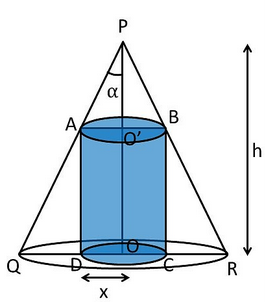
\includegraphics[scale=0.5]{figure.png}}\\
Figure.1
\end{center}

\section{Solution}
Given, Height of cone is 'h'.
\begin{align}
\implies h= \norm{\vec{P}-\vec{O}}
\end{align}
Let ,radius of cylinder be 'x'
\begin{align}
\implies x= \norm{\vec{A}-\vec{O^\prime}}=\norm{\vec{O^\prime}-\vec{B}}
\end{align}
From figure,
\begin{align}
\tan\alpha=\frac{\norm{\vec{A}-\vec{O^\prime}}}{\norm{\vec{P}-\vec{O^\prime}}}\\
\implies\norm{\vec{P}-\vec{O^\prime}}=x\cot\alpha
\end{align}
Height of cylinder say 'H' can be written as,
\begin{align}
H=\norm{\vec{O^\prime}-\vec{O}}=\norm{\vec{P}-\vec{O}}-\norm{\vec{P}-\vec{O^\prime}}\\
\implies H=h-x\cot\alpha
\end{align}
Volume of cylinder = (Area of base)x(Height of cylinder)
\begin{align}
V(x)=(\pi x^2) (h-x\cot\alpha)\\
\end{align}
\begin{center}
\textbf{objective function:}
\begin{align}
V= \max_\vec{x}\pi x^2(h-x\cot\alpha)\\
\end{align}
\textbf{constraints:}\\
x$>$0\\
h$>$0\\
0$<\alpha<$90\\
h, $\alpha$ are constants.
\end{center}
\begin{align}
\frac{dV(x)}{dx}=(2\pi xh)-(3\pi x^2 \cot\alpha)\\
\end{align}


Equating $\frac{dV(x)}{dx}$ to 0,
\begin{align}
  \implies x=\frac{2h}{3\cot\alpha}
\end{align}


Derivating equation (8) results,
\begin{align}
\frac{d^2 V(x)}{dx^2}=2\pi h-6\pi x\cot\alpha
\end{align}
putting (9) in (10) results,
\begin{align}
\frac{d^2 V(x)}{dx^2}=-2\pi h <0
\end{align}
$\therefore$ V(x) is maximum at $x=\frac{2h}{3\cot\alpha}$. \\
Equation (6)$\implies$
 Height of cylinder= $h-x\cot\alpha$.\\
\begin{align}
=h-\frac{2h}{3\cot\alpha}\cot\alpha\\
\implies H=\frac{h}{3}
\end{align}

$\therefore$ The height of the cylinder of maximum volume that can be inscribed in a cone of height h is $\frac{h}{3}$.

Volume of cylinder:-$V(x)=\pi x^2(h-x\cot\alpha)$\\


substitute equation (9) in above gives,
\begin{align}
V(x)=\pi \left(\frac{2h}{3\cot\alpha}\right)^2\left(h-\frac{2h}{3\cot\alpha}.\cot\alpha\right)\\
\implies V(x)=\frac{4}{27}\pi h^3\tan^2\alpha.
\end{align}

Let $\alpha=45\degree $ and 'h'=9.
\begin{align}
\implies V(x)=\pi x^2 (9-x)
\\ \frac{dV(x)}{dx}=18\pi x-3\pi x^2\\
\frac{dV(x)}{dx}=0 \implies x=6.\\
\frac{d^2V(x)}{dx^2}=18 \pi-6 \pi x\\
\end{align}
putting $x=6$ in above equation gives,
\begin{align}
\frac{d^2V(x)}{dx^2}=18\pi-36\pi=-18\pi <0.
\end{align}
$\therefore$ V(x) is maximum at $x=6$.\\
 Height of the cylinder (H)=$h-x\cot\alpha$\\
\begin{align}
\implies H=9-6\cot45\degree = 3 = \frac{1}{3}\text{ (Height of cone)}.
\end{align}
\textbf{Geometric programming:-}
\begin{align}
f(x)=\sum_{j=1}^{N} C_j  \prod_{i=1}^{n} x_i^{a_{ij}}\\
C_j >0 ,x_i\geq 0 ,a_{ij} \text{is real}.
\end{align}
Any non linear function which obeys the conditions in (28) can be solvable using geometric programming.
 
But , the function $V(x)$ have negative coefficient for $x^3$.

so ,we approximate the function $V(x)$ using the equations below.
\begin{align}
	f(w) \approx f(x)\prod_{i=1}^{n}\left({\frac{w_i}{x_i}}\right)^{a_i}
\end{align}
where
\begin{align}
	a_i = \frac{x_i}{f(x)}\frac{\partial{f}}{\partial{x_i}}
\end{align}
By keeping  the constraints like 
\begin{align}
x \geq \frac{x_k}{1+error}\\
x\leq (1+error)(x_k)
\end{align} 
where $x_k=x-10\delta$ ,

The above formulation can be iterated till the problem converges at a local maximum. Taking n = 1000 ,$\delta$= 0.001 and error=0.005 the optimal solution obtained
using cvxpy is
\begin{align*}
	\boxed{V_{max} = 339.3032173204817}\\
	\boxed{x = 6.022349936219689}
\end{align*}

\textbf{For Maxima :}
\\Using gradient ascent method,
\begin{align}
x_{n+1} = x_n + \alpha \nabla V(x_n)\\
\implies x_{n+1} = x_n + \alpha (3\pi x(6-x))
\end{align}
In equation (24), $\alpha$ is a variable parameter known as step size. $x_{n+1}$ is the next position.The positive sign refers to the maximization part of gradient ascent. By following the above method, we keep doing iterations until $x_{n+1}-x_n$ becomes
less than the value of precision.

Taking $\alpha$ = 0.001,$x_0$ = 2 and precision=0.00000001, values obtained using python are :
\begin{align*}
        \boxed{\text{Maxima} = 339.29200658769685 \approx 339 }\\
        \boxed{\text{Maxima Point} = 5.999999834068126 \approx 6}
\end{align*}
$\therefore$ Maxima value of $V(x)$ at $x=6$ is 339.\\
\begin{center}
{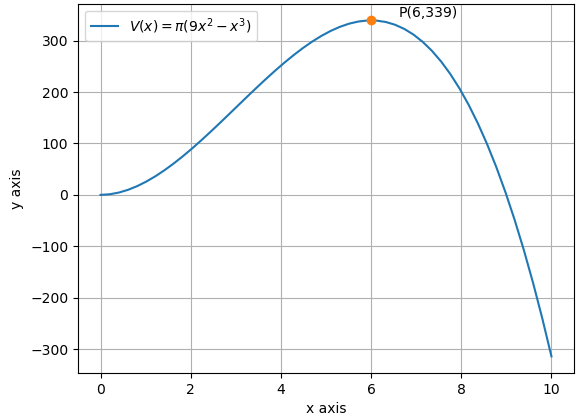
\includegraphics[scale=0.5]{graph.png}}\\
Figure.2:$V(x)=\pi x^2(9-x)$
\end{center} 
Below link shows python code to verify maxima of the function $V(x)$.
\begin{center}
\fbox{\parbox{8.5cm}{\url{https://github.com/FWC_module1/blob/main/optimization/advanced.py}}}
\end{center}

\end{document}